\documentclass{beamer}
\mode<presentation>
\usepackage{amsmath}
\usepackage{amssymb}
\usepackage{adjustbox}
\usepackage{subcaption}
\usepackage{enumitem}
\usepackage{multicol}
\usepackage{mathtools}
\usepackage{listings}
\usepackage{url}
\usepackage{minted}
\usepackage{tcolorbox}
\tcbuselibrary{minted,breakable,xparse,skins}

\definecolor{bg}{gray}{0.95}
\DeclareTCBListing{mintedbox}{O{}m!O{}}{%
  breakable=true,
  listing engine=minted,
  listing only,
  minted language=#2,
  minted style=default,
  minted options={%
    linenos,
    gobble=0,
    breaklines=true,
    fontsize=\scriptsize,
    numbersep=8pt,
    #1},
  boxsep=0pt,
  left skip=0pt,
  right skip=0pt,
  left=25pt,
  right=0pt,
  top=3pt,
  bottom=3pt,
  arc=5pt,
  leftrule=0pt,
  rightrule=0pt,
  bottomrule=2pt,
  toprule=2pt,
  colback=bg,
  colframe=orange!70,
  enhanced,
  overlay={%
    \begin{tcbclipinterior}
    \fill[orange!20!white] (frame.south west) rectangle ([xshift=20pt]frame.north west);
    \end{tcbclipinterior}},
  #3,
}

\def\UrlBreaks{\do\/\do-}
\usetheme{Madrid}
\usecolortheme{lily}
\setbeamertemplate{footline}
{
  \leavevmode%
  \hbox{%
  \begin{beamercolorbox}[wd=\paperwidth,ht=2.25ex,dp=1ex,right]{author in head/foot}%
    \insertframenumber{} / \inserttotalframenumber\hspace*{2ex} 
  \end{beamercolorbox}}%
  \vskip0pt%
}
\setbeamertemplate{navigation symbols}{}

\providecommand{\myvec}[1]{\ensuremath{\begin{pmatrix}#1\end{pmatrix}}}

\numberwithin{equation}{section}
\title{Matgeo Presentation}
\author{K. Akshay Teja \\ AI24BTECH11002\\IIT Hyderabad}
\date{November 5, 2024}

\begin{document}

\begin{frame}
    \titlepage
\end{frame}

\begin{frame}{Outline}
    \tableofcontents
\end{frame}

\section{Problem}
\begin{frame}{Problem Statement}
    Show that the points 
    \begin{align}
    P = \begin{pmatrix} -2 \\ 3 \\ 5 \end{pmatrix}, \quad Q = \begin{pmatrix} 1 \\ 2 \\ 3 \end{pmatrix}, \quad R = \begin{pmatrix} 7 \\ 0 \\ -1 \end{pmatrix}
    \end{align}
    are collinear.
\end{frame}

\section{Solution}


\subsection{Collinearity Condition}
\begin{frame}{Collinearity Condition}
    The points P, Q, and R are collinear if the vectors $ Q - P $ and $ R - P $ are linearly dependent. This is equivalent to the rank condition:
    \begin{align}
    \text{rank}\begin{pmatrix} Q - P & R - P \end{pmatrix} = 1
    \end{align}
\end{frame}

\subsection{Vector Calculation}
\begin{frame}{Vector Calculation}
    Calculate the vectors $ Q - P $ and $ R - P $:
    \begin{align}
    Q - P = \begin{pmatrix} 1 - (-2) \\ 2 - 3 \\ 3 - 5 \end{pmatrix} = \begin{pmatrix} 3 \\ -1 \\ -2 \end{pmatrix}, \quad R - P = \begin{pmatrix} 7 - (-2) \\ 0 - 3 \\ -1 - 5 \end{pmatrix} = \begin{pmatrix} 9 \\ -3 \\ -6 \end{pmatrix}
    \end{align}
\end{frame}

\subsection{Matrix and Row Reduction}
\begin{frame}{Matrix Row Reduction}
    Perform row reduction on the matrix:
    \begin{align}
    \begin{pmatrix} 3 & -1 & -2 \\ 9 & -3 & -6 \end{pmatrix} 
    \xrightarrow{R_2 \leftarrow R_2 - 3 R_1} \begin{pmatrix} 3 & -1 & -2 \\ 0 & 0 & 0 \end{pmatrix}
    \end{align}
    Since the matrix has a rank of 1, the points $ P $, $ Q $, and $ R $ are collinear.
\end{frame}

\section{Conclusion}
\begin{frame}{Conclusion}
    Since the matrix formed by $ Q - P $ and $ R - P $ has a rank of 1, the points $ P $, $ Q $, and $ R $ are collinear.
\end{frame}

\begin{frame}{Visualization}
    \begin{figure}
        \centering
        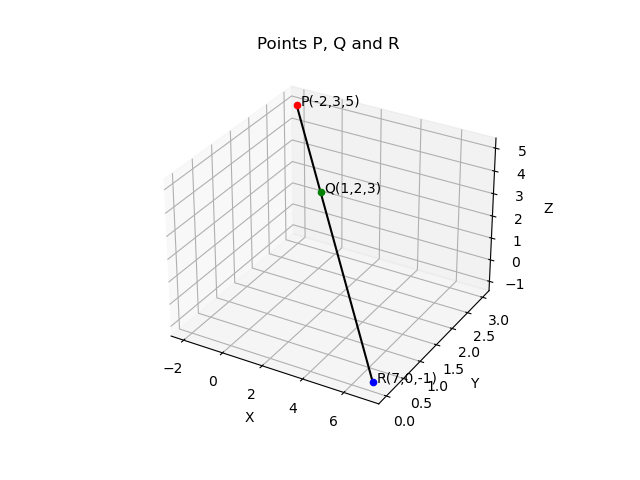
\includegraphics[width=0.8\textwidth]{fig/fig.png} 
	    \caption{Plot of Points P, Q, and R}
    \end{figure}
\end{frame}

\section{Codes}
\subsection{Generating Points on Line using C}

\begin{frame}[fragile,allowframebreaks]
\frametitle{Generating Points on Line using C}
\begin{mintedbox}{c}[break at=.8\textheight]
#include<stdio.h>

int main(){
	double P[]={-2,3,5},Q[]={1,2,3},R[]={7,0,-1};
	
	printf("P %.2lf %.2lf %.2lf\n",P[0],P[1],P[2]);
	printf("Q %.2lf %.2lf %.2lf\n",Q[0],Q[1],Q[2]);
	printf("R %.2lf %.2lf %.2lf\n",R[0],R[1],R[2]);
	int numberOfValues=100;

	double x_values[numberOfValues],y_values[numberOfValues],z_values[numberOfValues];

	for(int i=0;i<numberOfValues;i++){
		double t=(double)i/numberOfValues;
		x_values[i]=P[0]+t*(R[0]-P[0]);
		y_values[i]=P[1]+t*(R[1]-P[1]);
		z_values[i]=P[2]+t*(R[2]-P[2]);
	}
	for (int i = 0; i < numberOfValues; i++) {
        printf("%.2f %.2f %.2f\n", x_values[i], y_values[i], z_values[i]);
    }

    return 0;
}
\end{mintedbox}
\end{frame}

\subsection{Plotting the Figure using Python}
\begin{frame}[fragile,allowframebreaks]
\frametitle{Plotting the Figure using Python}
\begin{mintedbox}{Python}[break at=.8\textheight]
import numpy as np
import matplotlib.pyplot as plt
from mpl_toolkits.mplot3d import Axes3D
import subprocess

result = subprocess.run(['./code'],stdout = subprocess.PIPE,text=True)
output = result.stdout.strip().split('\n')

P = np.fromstring(output[0].replace('P ',''),sep=' ')
Q = np.fromstring(output[1].replace('Q ',''),sep=' ')
R = np.fromstring(output[2].replace('R ',''),sep=' ')

store=np.genfromtxt(output[3:],delimiter='')
x_values,y_values,z_values = store.T

fig = plt.figure()
ax = fig.add_subplot(111, projection='3d')

ax.scatter(*P, color='r', label='P')
ax.scatter(*Q, color='g', label='Q')
ax.scatter(*R, color='b', label='R')

ax.text(P[0]+0.2,P[1],P[2],'P(-2,3,5)',color='black', ha='left')
ax.text(Q[0]+0.2,Q[1],Q[2],'Q(1,2,3)',color='black', ha='left')
ax.text(R[0]+0.2,R[1],R[2],'R(7,0,-1)',color='black', ha='left')

ax.plot(x_values,y_values,z_values,color='k',label='Line through P,Q,R')

ax.set_xlabel('X')
ax.set_ylabel('Y')
ax.set_zlabel('Z')

plt.title('Points P, Q and R')
plt.grid(True)
plt.savefig('/home/akshay-teja-kondi/gvv/Assignment3/fig/fig.png')
\end{mintedbox}
\end{frame}

\end{document}
